The insights from~\Cref{sec:insights} emphasize the importance of tuning with API usage examples, in-context demonstration and generation regulation in the domain of tool manipulation. In this section, \emph{we revisit three techniques from the LLM literature and adapt them to address the aforementioned challenges, using a practical amount of human supervision}. 
% In this section, we introduce three simple techniques to implement the three insights from~\Cref{sec:insights} on top of open-source LLMs. 
We first introduce model alignment with programatically curated data to internalize API usage knowledge in~\Cref{subset:model_align}. We then discuss augmenting open-source LLMs with an in-context demonstration retriever in~\Cref{subset:demo_retrieve}. Lastly, we apply a system prompt to regulate generation in~\Cref{subset:sysprompt}.
% We first apply a fixed system prompt to instruct the model to only generate API calls. 
% To improve argument filling with in-context demonstrations, we augment LLMs with a retriever which selects relevant examples from a small human-curated set. 
% Finally we bake in example usage through multi-task instruction tuning to enhance API selection; we programmatically generate these examples from human-written templates to ensure minimal supervision. 
These techniques collectively serve as a strong baseline for alleviating the challenges presented in~\Cref{sec:insights} and inspiring further innovations.
% and inspire further innovations for open-source LLMs. 

\subsection{Multi-tool model alignment with programmatic data curation}
% \paragraph{Model alignment with programmatic data curation}
\label{subset:model_align}

Model alignment, through tuning LLMs with usage examples, plays a vital role in improving LLMs for capabilities such as instruction following and conversation~\cite{ouyang2022training, glaese2022improving, chung2022scaling}. 
% By tuning LLMs with usage examples, model alignment enhances the generation behavior towards targeted capabilities. 
In light of our insights from in~\Cref{sec:insights}, we recognize the potential of model alignment with API usage examples to improve API selection capability. To practically leverage such alignment for tool manipulation, it requires a data curation strategy without massive manual example writing. Towards this end, we prototype a method which generates usage examples from human-curated templates.

\begin{wrapfigure}[18]{r}{5.8cm}
\vspace{-12pt}
\caption{Programmatic training data generation using templates and random values}\label{fig:data_gen}
\centering
\vspace{-6pt}
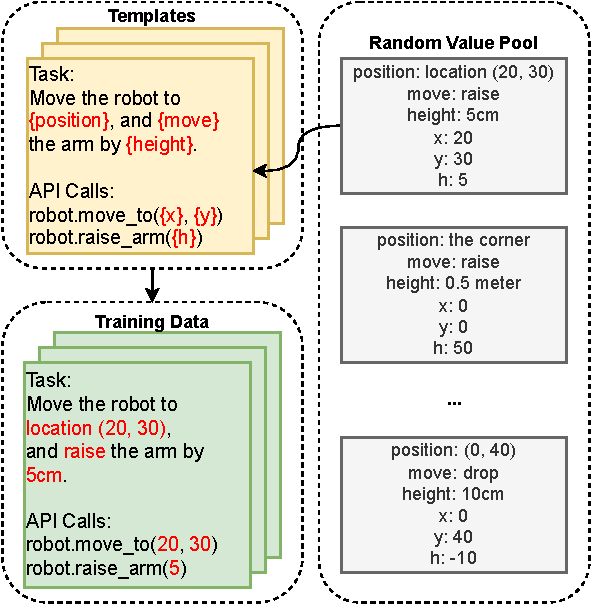
\includegraphics[width=\linewidth]{plots/data_gen.pdf}
\end{wrapfigure} 
% \paragraph{Data curation} 
\Cref{fig:data_gen} depicts our flow to generate alignment data.
We create a handful of templates consisting of goal descriptions and corresponding API calls. 
These templates contain one or more placeholder pairs. Each of these pairs maps to a key word in the goal and an argument in the corresponding API calls. 
We also provide a pool of candidate values for each keyword and randomly choose values to fill in the placeholders within the template. 
% This template instantiation process  process results in the instantiation of the goal description template and the generation of one or a sequence of API calls, with their arguments filled in with the corresponding values. 
Given a tool with $n$ candidate APIs, we only require $\mathcal{O}(n)$ human-curated templates to ensure practical human supervision. Specifically we use a principle where each of the $n$ APIs is encouraged to appear in at least one template. 
In practice, we find it takes on average one day for one developer to curate the data for one software tool in our benchmark; this includes writing the goal templates, providing the pool of argument values and generate the data. We provide example templates we use for different tools in~\Cref{sec:app_exp_details}. 
With data curated for all the tools, we perform model alignment tuning \emph{jointly for all tools and produce a single model}.




% Model alignment great in many stuff. 
% Alignment is very useful to help API selection.
% To implement model alignment which can practically used for developers on tool manipulation, Diversity is important, but how to avoid hand writting tons of usage examples.

% Instead of writing usage examples directly, we write a handful of goal descriptions in different wording, we then super charge by swapping the key words / arguments. 

\subsection{Demonstration retrieval}
% \paragraph{Demonstration retrieval}
\label{subset:demo_retrieve}


In~\Cref{sec:insights}, we demonstrate the efficacy of hand-picked oracle examples in improving argument populating. However, extending from oracles to practical in-context demonstration poses two challenges. First, given $n$ API function candidates, there are exponentially many combinations of API calls associated with different goals. Thus, LLMs should be capable of generalizing to a wide variety of goals based on a limited number of examples. Second, to ensure effective demonstration, it is important to provide LLMs with only the relevant examples without human interventions.

To fulfill the above two desiderata, we augment open-source LLMs with a demonstration retriever module. This module revolves around a repository where every API is required to appear in only one human-curated demonstration. This implies that only $\mathcal{O}(n)$ examples are needed. 
% On top of these demonstration examples, we use a ranker $\mathcal{R}_e$ to sort and return the examples with the most semantically similar goal descriptions. As the retriever only requires $\mathcal{O}(n)$ human-curated demonstrations, it could empower LLMs to manipulate tools over a large API combination space with a practical amount of human supervision.
Among these demonstration examples, the retriever selects the most semantically similar examples to the goal descriptions.
% We've shown that adding a single demonstration example can boost the model accuracy by a lot, but there are 2 practical concerns: 1) When a request needs to use a combination of multiple API functions, the oracle example may not exist, unless the example set exhausts all the possible combinations. This requires the example set to grow exponentially as the number of API functions increases; 2) Even if the oracle example exists, there is no guarantee that we can always get the oracle examples from the example set. 

\begin{wrapfigure}[13]{r}{5.5cm}
\vspace{-12pt}
\caption{In-context demonstration can improve both closed and open-source models on Home Search, a tool for browsing houses on sale.}\label{fig:demo_retrieve}
\vspace{-4pt}
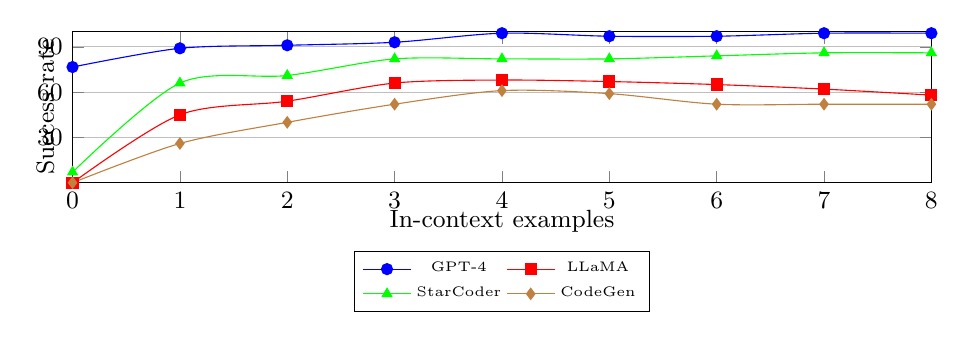
\begin{tikzpicture}
    \begin{axis}[
        xlabel=$x$,
        ylabel=$y$,
        xmin=0, xmax=8,
        ymin=0, ymax=100,
        xtick={0, 1, 2, 3, 4, 5, 6, 7, 8},
        ytick={30,60,90},
        % ytick={20,40,60,80,100},
        width=1.03\linewidth, height=3.5cm,
	ylabel=Success rate,
	ymajorgrids,
        y tick label style={font=\small},
        y label style={yshift=-3ex, font=\small},
	xlabel=In-context examples,
        x tick label style={font=\small},
        x label style={yshift=1.5ex, font=\small},
        legend style={
            at={(0.5,-0.45)},
            anchor=north,
            legend columns=2,
            font=\tiny,
            /tikz/every even column/.append style={column sep=0.cm},
        },
    ]
    \addplot[smooth,mark=*,blue] plot coordinates {
        (0,76.6)
        (1,89)
        (2,91)
        (3,93)
        (4,99)
        (5,97)
        (6,97)
        (7,99)
        (8,99)
    };
    \addlegendentry{GPT-4}

    \addplot[smooth,color=red,mark=square*]
        plot coordinates {
        (0,0)
        (1,45)
        (2,54)
        (3,66)
        (4,68)
        (5,67)
        (6,65)
        (7,62)
        (8,58)
    };
    \addlegendentry{LLaMA}
    % \addlegendentry{LLaMA-30b}

    \addplot[smooth,color=green,mark=triangle*]
        plot coordinates {
        (0,7)
        (1,66)
        (2,71)
        (3,82)
        (4,82)
        (5,82)
        (6,84)
        (7,86)
        (8,86)
    };
    \addlegendentry{StarCoder}

    % \addplot[smooth,color=green,mark=triangle*]
    %     plot coordinates {
    %     (0,0)
    %     (1,10)
    %     (2,19)
    %     (3,21)
    %     (4,17)
    %     (5,22)
    %     (6,20)
    %     (7,18)
    %     (8,17)
    % };
    % \addlegendentry{NeoX-20b}

    \addplot[smooth,color=brown,mark=diamond*]
        plot coordinates {
        (0,0)
        (1,26)
        (2,40)
        (3,52)
        (4,61)
        (5,59)
        (6,52)
        (7,52)
        (8,52)
    };
    \addlegendentry{CodeGen}
    % \addlegendentry{CodeGen-16b-mono}
    \end{axis}
\end{tikzpicture}
\end{wrapfigure} 
\paragraph{Validation} 
To verify the effectiveness of demonstration examples in practice, we empirically show that the retrieved demonstrations can improve the success rate on goals requiring API combinations unseen in the example repository. 
In particular, we evaluate this approach on the home search task which exposes $15$ API functions and requires multiple functions to accomplish each goal. With only $10$ human-curated demonstrations that do not precisely match any of the $100$ test cases in terms of API combinations, the retrieved demonstrations can boost the success rate by up to $79\%$ across open-source LLMs and make GPT-4 nearly perfect, as shown in \Cref{fig:demo_retrieve}. This shows that the demonstration examples can improve tool manipulation for unseen types of goals with a repository of size $\mathcal{O}(n)$ only.
% In particular, we use the same test set of Home Search, but when designing the few-shot examples, we explicitly make sure that the API combination of each test case never appears in the training examples. We can clearly see the answers to the above concerns with the results in Figure \ref{fig:tech_1}. First, using retrieved examples can still bump up the model accuracy significantly. Second, the accuracy saturates quickly as the number of examples increases, indicating that the models are able to generalize beyond the examples to the broader unseen combinations with limited demonstrations.
% \comment{QT: please correct facts and numbers here}



% In this section, we proposed several simple techniques in accordance to the findings in section \ref{sec:insights}. We conducted experiments to validate if they can boost the model performance. 

% 3 techniques which make conventional NLP great. Adapt these techniques to tool manipulation with very minimal human super vision.

\subsection{Generation regulation with system prompts}
% \paragraph{Generation regulation with system prompts}
\label{subset:sysprompt}

\begin{wrapfigure}[17]{r}{6.2cm}
\vspace{-12pt}
\caption{System prompt with guidelines to only generate code in a desired format. Red parts are populated with real data for each test case during inference.}
\vspace{-5pt}
\label{fig:sysprompt}
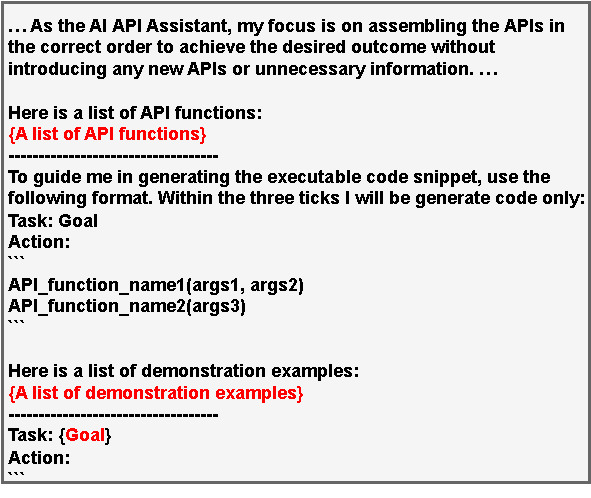
\includegraphics[width=\linewidth]{plots/sys_prompt_full.pdf}
% 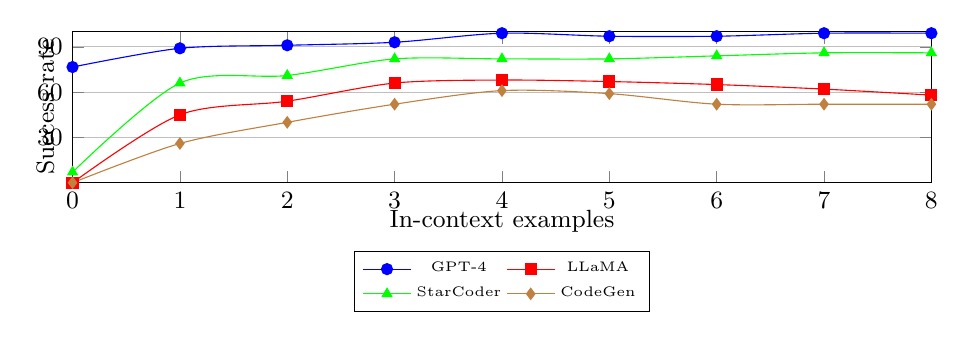
\begin{tikzpicture}
    \begin{axis}[
        xlabel=$x$,
        ylabel=$y$,
        xmin=0, xmax=8,
        ymin=0, ymax=100,
        xtick={0, 1, 2, 3, 4, 5, 6, 7, 8},
        ytick={30,60,90},
        % ytick={20,40,60,80,100},
        width=1.03\linewidth, height=3.5cm,
	ylabel=Success rate,
	ymajorgrids,
        y tick label style={font=\small},
        y label style={yshift=-3ex, font=\small},
	xlabel=In-context examples,
        x tick label style={font=\small},
        x label style={yshift=1.5ex, font=\small},
        legend style={
            at={(0.5,-0.45)},
            anchor=north,
            legend columns=2,
            font=\tiny,
            /tikz/every even column/.append style={column sep=0.cm},
        },
    ]
    \addplot[smooth,mark=*,blue] plot coordinates {
        (0,76.6)
        (1,89)
        (2,91)
        (3,93)
        (4,99)
        (5,97)
        (6,97)
        (7,99)
        (8,99)
    };
    \addlegendentry{GPT-4}

    \addplot[smooth,color=red,mark=square*]
        plot coordinates {
        (0,0)
        (1,45)
        (2,54)
        (3,66)
        (4,68)
        (5,67)
        (6,65)
        (7,62)
        (8,58)
    };
    \addlegendentry{LLaMA}
    % \addlegendentry{LLaMA-30b}

    \addplot[smooth,color=green,mark=triangle*]
        plot coordinates {
        (0,7)
        (1,66)
        (2,71)
        (3,82)
        (4,82)
        (5,82)
        (6,84)
        (7,86)
        (8,86)
    };
    \addlegendentry{StarCoder}

    % \addplot[smooth,color=green,mark=triangle*]
    %     plot coordinates {
    %     (0,0)
    %     (1,10)
    %     (2,19)
    %     (3,21)
    %     (4,17)
    %     (5,22)
    %     (6,20)
    %     (7,18)
    %     (8,17)
    % };
    % \addlegendentry{NeoX-20b}

    \addplot[smooth,color=brown,mark=diamond*]
        plot coordinates {
        (0,0)
        (1,26)
        (2,40)
        (3,52)
        (4,61)
        (5,59)
        (6,52)
        (7,52)
        (8,52)
    };
    \addlegendentry{CodeGen}
    % \addlegendentry{CodeGen-16b-mono}
    \end{axis}
\end{tikzpicture}
\end{wrapfigure} 
The use of system prompts is a well-established technique in chatbots powered by LLMs~\cite{glaese2022improving}. By incorporating human-chatbot conversations, system prompts can effectively control the natural language style of the generated responses. In the context of tool manipulation, we regularize open-source LLMs to exclusively generate API calls with a system prompt in~\Cref{fig:sysprompt}, where the black part is the template shared across all tasks and the red rows are instantiated during inference for a certain goal. Our system prompt first defines a format that combines text sections containing goals, demonstrations, and generations. It then provides explicit guidelines in natural language, instructing the LLMs to generate code exclusively. The system prompt incorporates the goal description and the retrieved API functions directly for each request, reducing the human development effort to a one-time task. 
% \comment{QT: Lets insert the example visual of a system prompt.}
% \begin{wrapfigure}[]{r}{5.5cm}
% \vspace{-20pt}
% \caption{(place holder) with or without restriction vs acc on the OpenwWeather}\label{fig:tech_2}
% \includegraphics[width=5.5cm]{plots/tech_2.png}
% \end{wrapfigure} 

% To verify the hypothesis, we compare two different types of queries on the OpenWeather, where the only difference is if there is an extra phrase "(answer in code only)" appended in the end of the prompt or not. As shown in  Figure \ref{fig:tech_2}, adding "(answer in code only)" in prompt greatly regularized the output to our expected format, so as to greatly improve the model accuracy, indicating that regularize the model output is effective in boosting model accuracy.
% \comment{Fenglu, describe the results}
% 1. Different questions doesn't matter.
% 2. Adding "(answer in code only)" in prompt greatly regularized the output to our expected format, so as to greatly improve the model accuracy.


% This observation of the LLMs benefits a lot from regularizing the output formats further motivates us to explore system prompt\cite{}. \comment{Changran, more reference, more results}
% General good system prompt HHH
% You are careful, you follow the instructions
% Task specific task prompt 
% For redfin, you are a good house hunter assistant
% Better describe what should be generated as the output
% Api call only
% ```stuff ```
% Only use API that is provided
% If API provided not enough, refuse to answer



% A straight forward extension is to include more demonstration examples in the prompt, so as to have more chance of covering the real use case of a given input request. But this raises another issue about \emph{how to gather the most relevant examples for a given request}. For now we use the BM25 retriever in all our experiments. It is effective, but still makes mistakes and usually the LLM has no chance to generate correct actions based on mistakenly retrieved API functions or examples. We leave the retrieval improvement to future works.

 



% \begin{wrapfigure}[]{r}{5.5cm}
% \vspace{-20pt}
% \caption{(place holder) acc of tuned models on open weather and booking}\label{fig:tech_3}
% \includegraphics[width=5.5cm]{plots/tech_3.png}
% \end{wrapfigure} 
% With the observation that baking API usage information in the model helps the practical action generation, we want to further bump the public LLM's accuracy to match the closed-source models. In particular, we manually created small amount of training data and finetuned Pythia-12b\cite{biderman2023pythia} on 2 tasks: Open Weather and Trip Booking.  
% \comment{Fenglu, data details, amount + creating method} 10 manually created templates * 50 samples with random fill-in values. Avoid test set leakage.

% As shown in Figure \ref{fig:tech_3}, after finetuning a model on a given task, its accuracy on that task can be greatly improved and the gap between gpt-3.5 is greatly reduced. 
% \comment{TODO: Following studies about the synergy between training on different tasks.}


% We found that though the models have great language understanding capability, instruction following ability, and basic knowledge of API calls, without specific tuning, it is still likely to fail to generate correct API calls. In most cases, it can get the component correctly, but will fail because the lack of mastering the exact grammar and/or subtle usage of the API's. For example XXXX

% We aggregate the above three techniques to further enhance tool manipulation. Specifically we first tune open-source LLMs without a system prompt or a demonstration retriever. During inference, we enable both techniques to maximize the tool manipulation capability.
% \comment{QT: Lets discuss and see if to provide a diagram to explan the full system for its train time and inference time pipeline with all these 3 techniques turned on.}
